\chapter{Methode}
In dit hoofdstuk wordt het ontwerp van de pipet en de realisatie ervan besproken. Hierbij worden de verschillende onderdelen behandeld, alsook de gemaakte keuzes.

\section{Conceptueel ontwerp}
De literatuurstudie richt zich sterk op bestaande patenten. Zo beschrijven Al-Mahareeq en Al-Mahrouq Hasan~\cite{RN17} en Shapiro~\cite{RN16} (beiden vervallen) manueel bediende, analoge pipetten met een eenvoudige zuigerwerking. Deze vormen een waardevolle basis voor het begrijpen van de fundamentele werking, die essentieel is bij het ontwerp van een automatische pipet.
\\\textit{Zie \autoref{sec: Analoge pipetten} voor verdere toelichting betreffende de werking.}
\\[12pt]Daarnaast beschrijven Nelson et al., Lind et al.\ en Solotareff et al.\cite{RN35,RN36,RN38} elektronische, motorisch aangedreven pipetten. In het werk van Nelson et al.~\cite{RN35} wordt expliciet het gebruik van een stappermotor vermeld, wat bevestigt dat nauwkeurige zuigersturing mogelijk is met dit type motor. Van deze patenten is enkel dat van Lind en Pekkanen (2019)~\cite{RN36} nog actief. Dit patent beschrijft hoe een elektrische motor als aandrijving wordt toegepast. Dit concept is echter niet uniek aan hun werk en heeft geen directe impact op het ontwerp in deze thesis. Het patent van Nelson et al. is eveneens nog actief, maar lijkt niet meer onderhouden te worden.

\section{MOSCOW-analyse}
In Tabel~\ref{tab:moscow} worden de vereisten voor het pipetteersysteem samengevat volgens het MOSCOW-principe. De eisen zijn geclusterd in \textit{Must have}, \textit{Should have}, \textit{Could have} en \textit{Won’t have} elementen, en vormen samen de functionele en ontwerptechnische randvoorwaarden van deze thesis.

\begin{table}[H]
    \centering
    \caption{MOSCOW-analyse voor het pipetteersysteem}\label{tab:moscow}
    \begin{tabularx}{\textwidth}{|l|X|}
        \hline
        \textbf{Categorie} & \textbf{Vereisten} \\
        \hline
        \textbf{Must have} & 
        \begin{itemize}
            \item Reproduceerbare pipetteerhandelingen conform ISO 8655--2
            \item Instelbare en programmeerbare volumeregeling
            \item Modulair ontwerp met uitbreidingsmogelijkheden
            \item Compatibiliteit met standaard laboratoriumspuiten
        \end{itemize} \\
        \hline
        \textbf{Should have} & 
        \begin{itemize}
            \item Stil en nauwkeurig mechanisch functioneren
            \item Softwarematige controle via een programmeerbare interface (API)
            \item Beperkte trillingen en stabiele, lineaire beweging
            \item Materiaal- en bouwkosten binnen bereik van kleinschalige laboratoria
        \end{itemize} \\
        \hline
        \textbf{Could have} & 
        \begin{itemize}
            \item Feedback-systeem voor positienauwkeurigheid
            \item Ondersteuning voor multi-channel pipetteren
            \item Validatie met biologische monsters
            \item Integratie in geautomatiseerde liquid handling systemen
        \end{itemize} \\
        \hline
        \textbf{Won’t have (in huidige versie)} & 
        \begin{itemize}
            \item Directe volumemeting tijdens pipetteren
        \end{itemize} \\
        \hline
    \end{tabularx}
\end{table}

\subsection{Wandelementen}
Zoals eerder vermeld, is voor een modulair hardwareontwerp gekozen. Dit maakt het mogelijk om onderdelen afzonderlijk te ontwikkelen, aan te passen of in de toekomst uit te breiden naar bijvoorbeeld een meerkanalensysteem. De modules worden op geleidestaven geplaatst, zoals te zien in \autoref{fig:geleidestaven}, wat zorgt voor correcte uitlijning.
De wanden zijn 3D-geprint in PLA, wat volstaat gezien de beperkte structurele belasting. 
\\[12pt]In latere iteraties zijn de wanden lichter en goedkoper gemaakt door de wanden te verdunnen en vlakken te verwijderen (\autoref{fig:dubbelemuur}). Er zijn wandelementen van 80 mm en 30 mm ontworpen met een parametrisch model. Aanvankelijk bestond het 80 mm element uit twee delen van 40 mm, maar deze verbinding zorgde voor een naad waar de geleideslede moeilijk voorbij kon. Daarom is gekozen voor één geheel, wat de werking van de geleideslede verbetert.
\\[12pt]\begin{minipage}[t]{0.49\textwidth}
    \vspace{0pt}
    \begin{figure}[H]
        \centering
        \captionsetup{width=1\textwidth} % wider caption box
        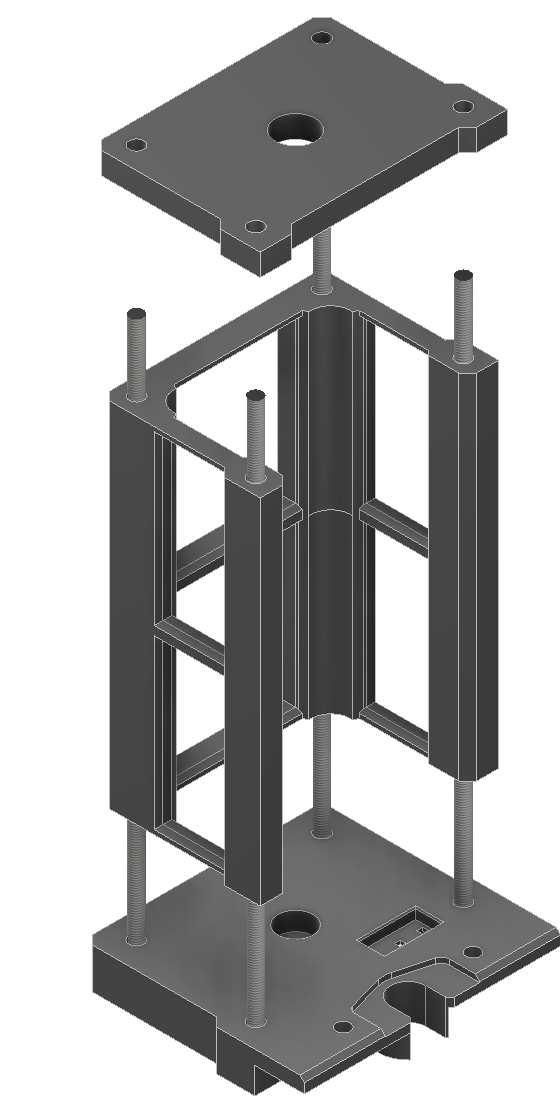
\includegraphics[height=6cm]{figures/GuidesDemonstration_2.png}
        \caption{Demonstratie van de geleidestaven}\label{fig:geleidestaven}
    \end{figure}
\end{minipage}
\begin{minipage}[t]{0.49\textwidth}
    \vspace{0pt}
    \begin{figure}[H]
        \centering
        \captionsetup{width=1\textwidth} % wider caption box
        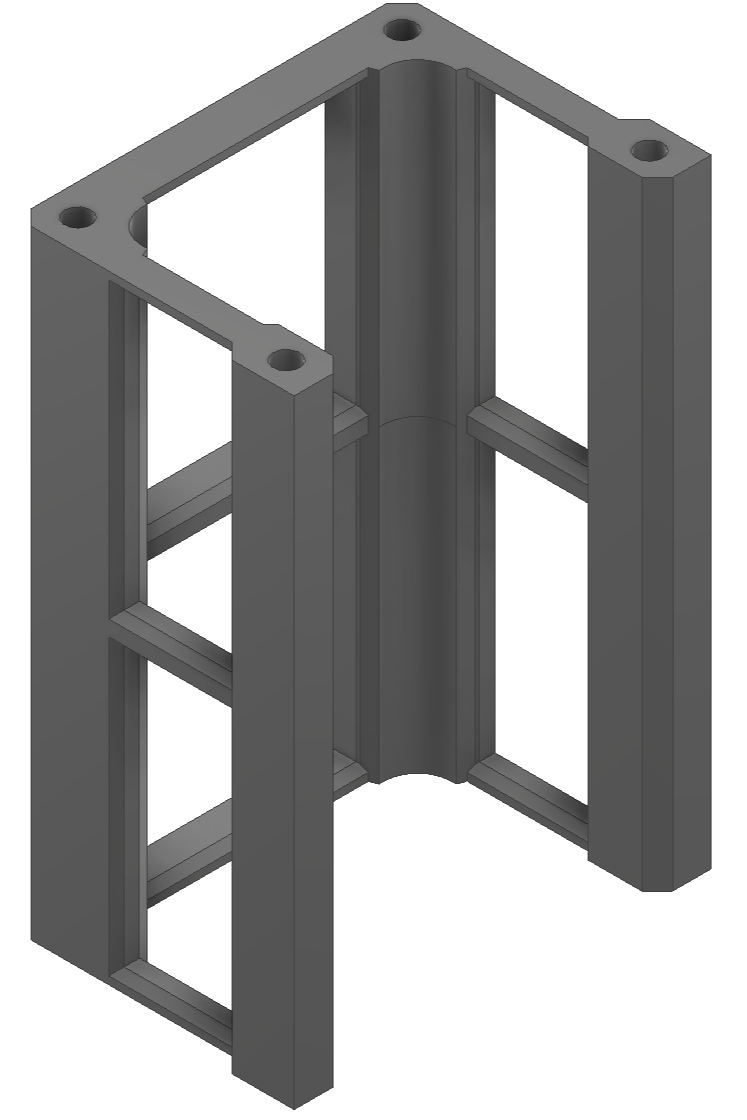
\includegraphics[height=6cm]{figures/Wall_2_w.png}
        \caption{Verdubbeld wandelement}\label{fig:dubbelemuur}
    \end{figure}
\end{minipage}\\

\subsection{Bodemplaat en geleidestaven}
De wandelementen en geleidestaven worden gemonteerd op de bodemplaat, die voorzien is van gaten voor de geleidestaven. Aan de onderzijde worden tegengedraaide moeren gebruikt, een methode die ook voorkomt bij de montage van verkeerslichten (\autoref{fig:verkeerslichten}) en in\ \cite{RN40}. Deze techniek verstevigt 3D-geprinte onderdelen en maakt montage in segmenten mogelijk.
\\[12pt]De gebruikte moeren (ISO 4032-M3) passen in speciaal ontworpen gaten (\autoref{fig:counterrotated}) met twee trappen: een onderste zeskantvormige uitsparing waarin de moer net past en nauwelijks kan roteren, en een cilindrische bovenste trap voor plaatsing van de tweede moer. Deze wordt aangedraaid, zodat beide moeren stevig vastzitten en niet kunnen verdraaien. Door hiervoor tegengedraaide moeren te gebruiken kunnen deze achteraf gedemonteerd worden.
\\[12pt]\begin{minipage}[t]{0.49\textwidth}
    \vspace{0pt}
    \begin{figure}[H]
        \centering
        \captionsetup{width=1\textwidth} % wider caption box
        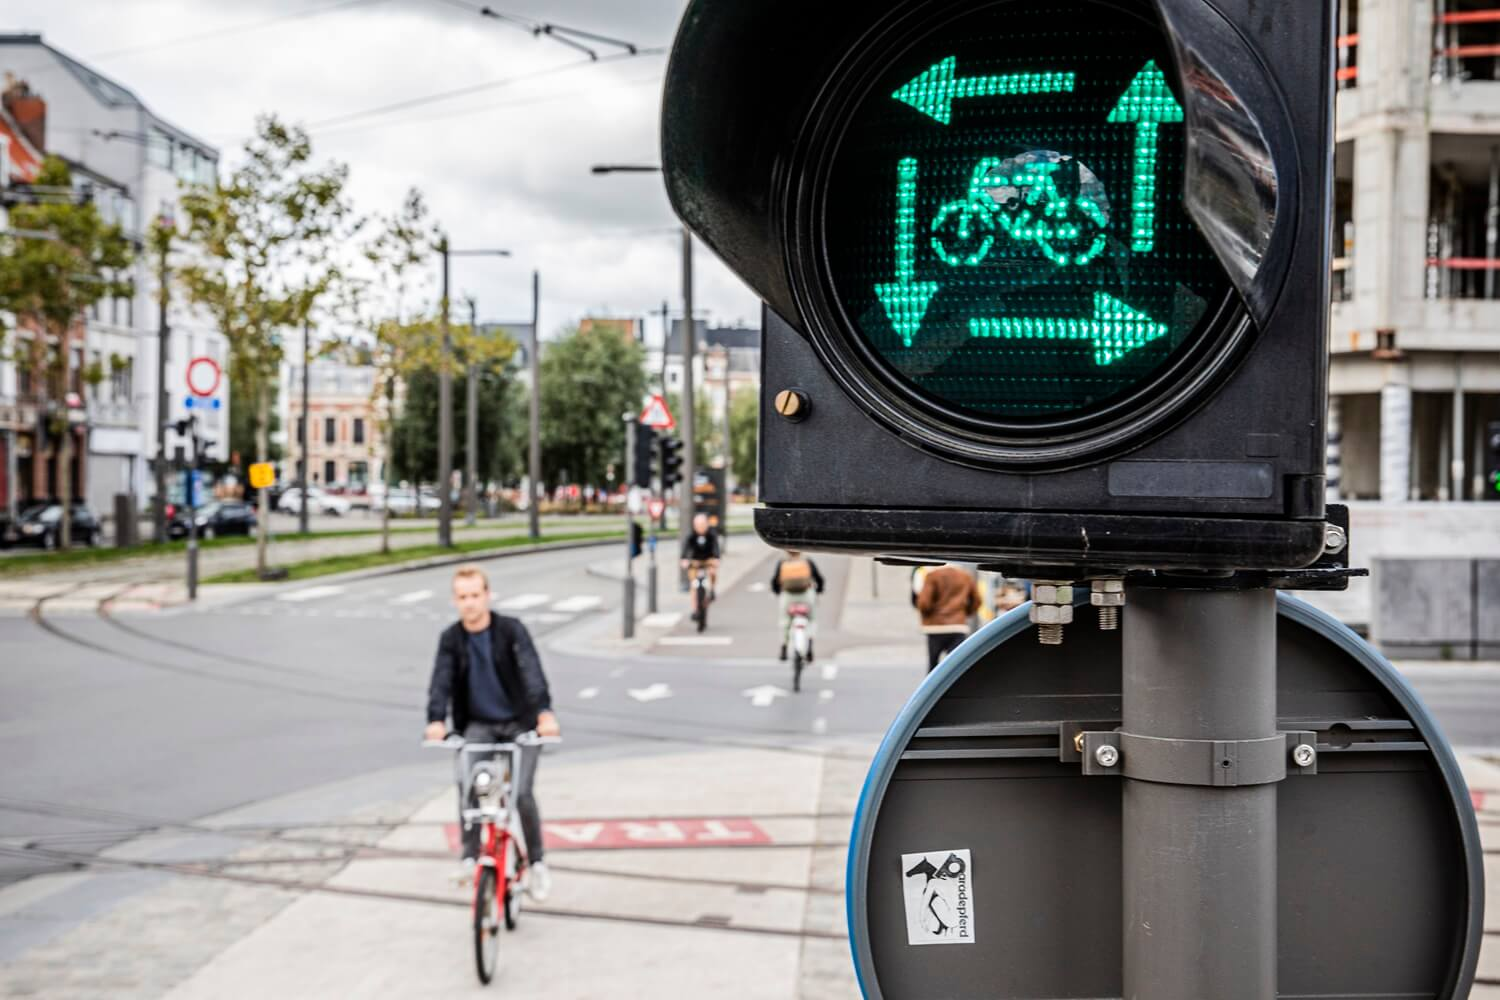
\includegraphics[height=4cm]{figures/verkeerssituaties48.jpg}
        \caption{Montage van verkeerslichten}\label{fig:verkeerslichten}
        \textbf{Bron}: uitgesneden uit\ \cite{RN39}
    \end{figure}
\end{minipage}
\begin{minipage}[t]{0.49\textwidth}
    \begin{figure}[H]
        \centering
        \captionsetup{width=1\textwidth} % wider caption box
        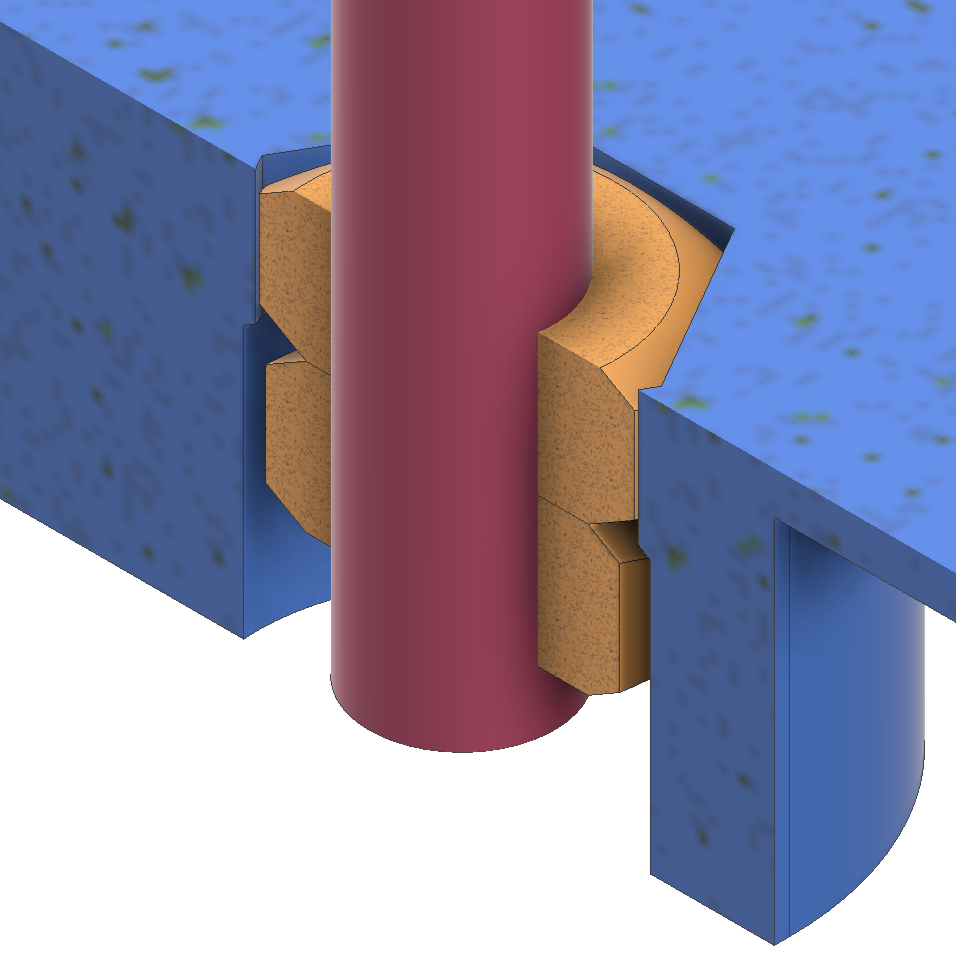
\includegraphics[height=4cm]{figures/InterlockingScrews.png}
        \caption{Tegengedraaide moeren}\label{fig:counterrotated}
    \end{figure}
\end{minipage}\\[12pt]
De bodemplaat is voorzien van verschillende gaten en uitsparingen zoals te zien in\ \autoref{fig:bodemplaat}. Zo zijn er vier gaten voor de geleidestaven. Ook is er een grote centrale opening voor de loodschroef. Hierin past een lager van formaat ID:4mm, OD:8mm. Verder is er een uitsparing waarin een eindeloopschakelaar past. Aan de rand is er een uitsparing waar de spuit in past. Rond deze uitsparing is er een verlaging waarin de grepen van de spuit passen. Dit alles wordt met een klem (\autoref{fig:clamp}) vastgehouden doorheen de beweging. Deze klem past in de uitsparing en wordt vastgezet met twee M3 schroeven en moeren door de daarvoor voorziene gaten.
\\[12pt]\begin{minipage}[t]{0.49\textwidth}
    \vspace{0pt}
    \begin{figure}[H]
        \centering
        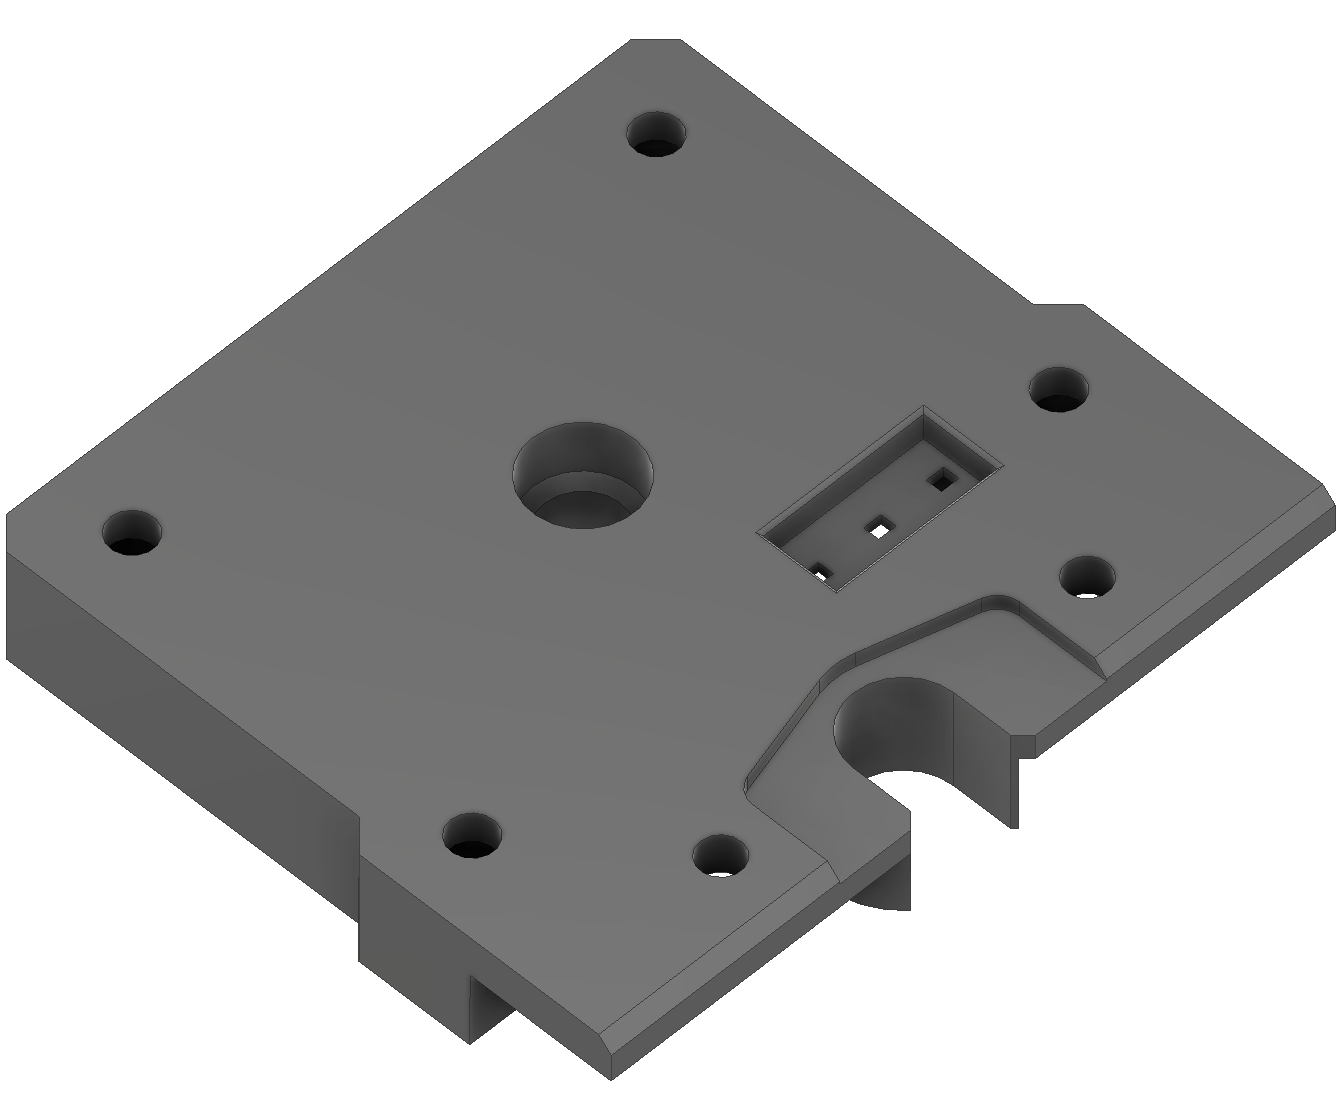
\includegraphics[height=4cm]{figures/Foundation_1_w.png}
        \caption{Bodemplaat}\label{fig:bodemplaat}
    \end{figure}
\end{minipage}
\begin{minipage}[t]{0.49\textwidth}
    \vspace{0pt}
    \begin{figure}[H]
        \centering
        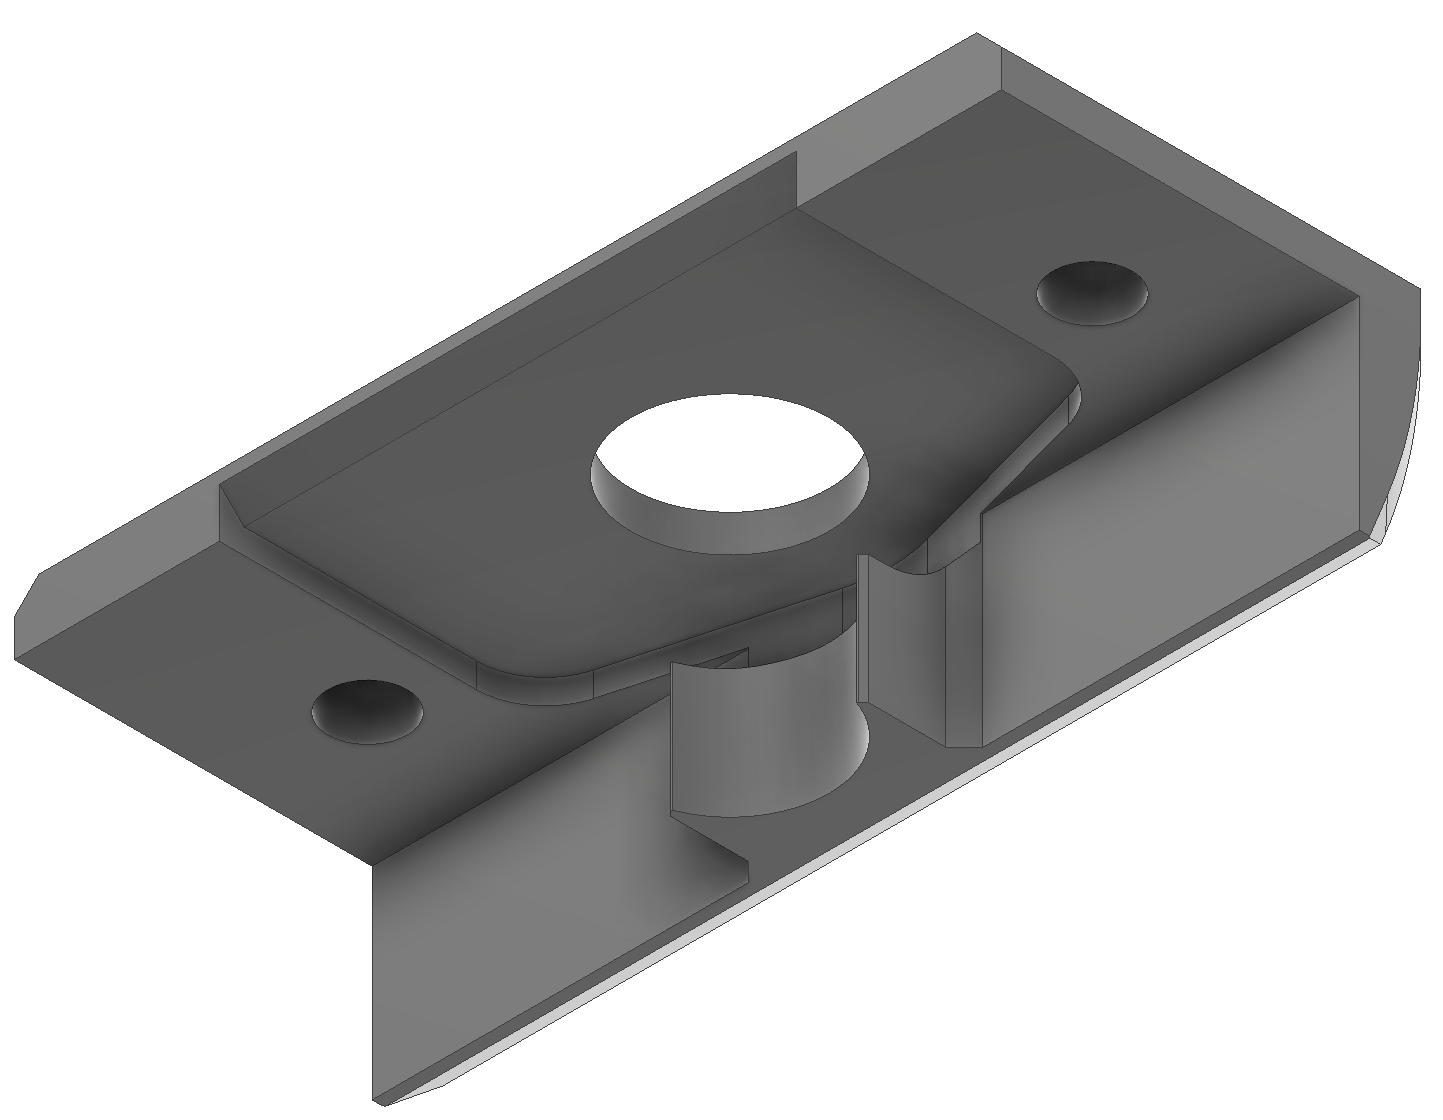
\includegraphics[height=4cm]{figures/Foundation_clamp_w.png}
        \caption{Klem spuit (zuiger)}\label{fig:clamp}
    \end{figure}
\end{minipage}\\

\subsection{Tussenplaat en motorplaat}
Deze twee platen passen tussen de wandelementen. De tussenplaat (\autoref{fig:tussenplaat}) vormt de grens tussen de askoppeling en de zuigerkamer. De motorplaat (\autoref{fig:motorplaat}) bevindt zich bovenaan en heeft een uitsparing voor een Nema 8 stappermotor die met M2 schroeven bevestigd wordt. 
\\[12pt]\begin{minipage}[t]{0.49\textwidth}
    \vspace{0pt}
    \begin{figure}[H]
        \centering
        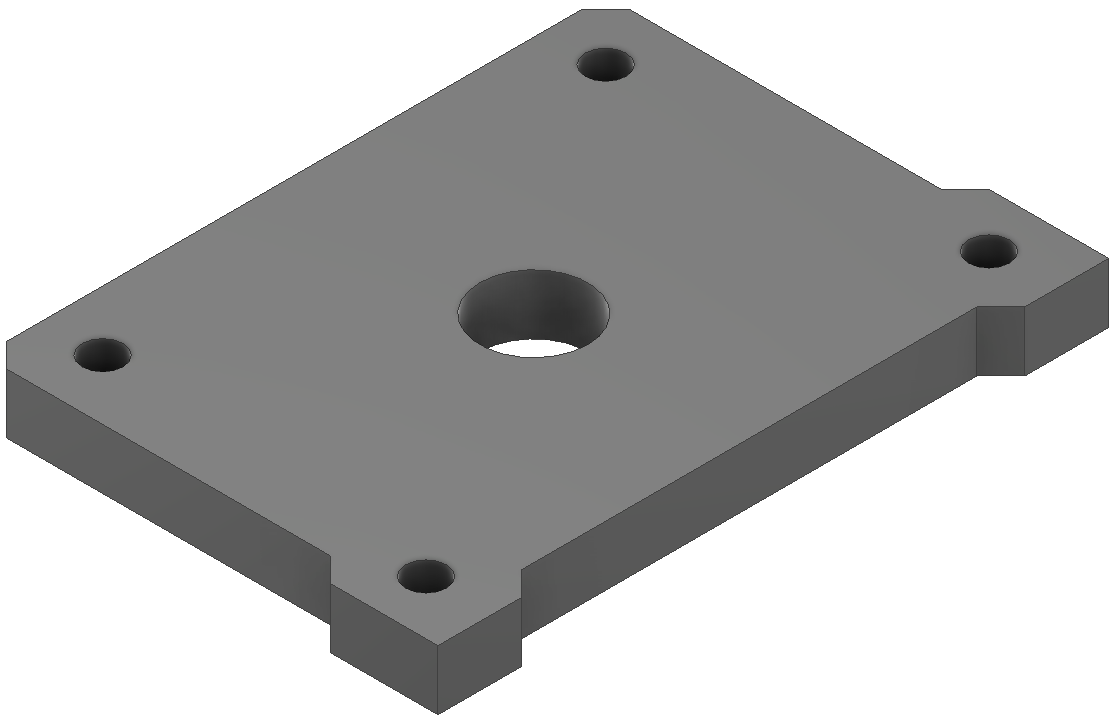
\includegraphics[width=0.65\textwidth]{figures/Topp_Wall_w.png}
        \caption{Tussenplaat}\label{fig:tussenplaat}
    \end{figure}
\end{minipage}
\begin{minipage}[t]{0.49\textwidth}
    \vspace{0pt}
    \begin{figure}[H]
        \centering
        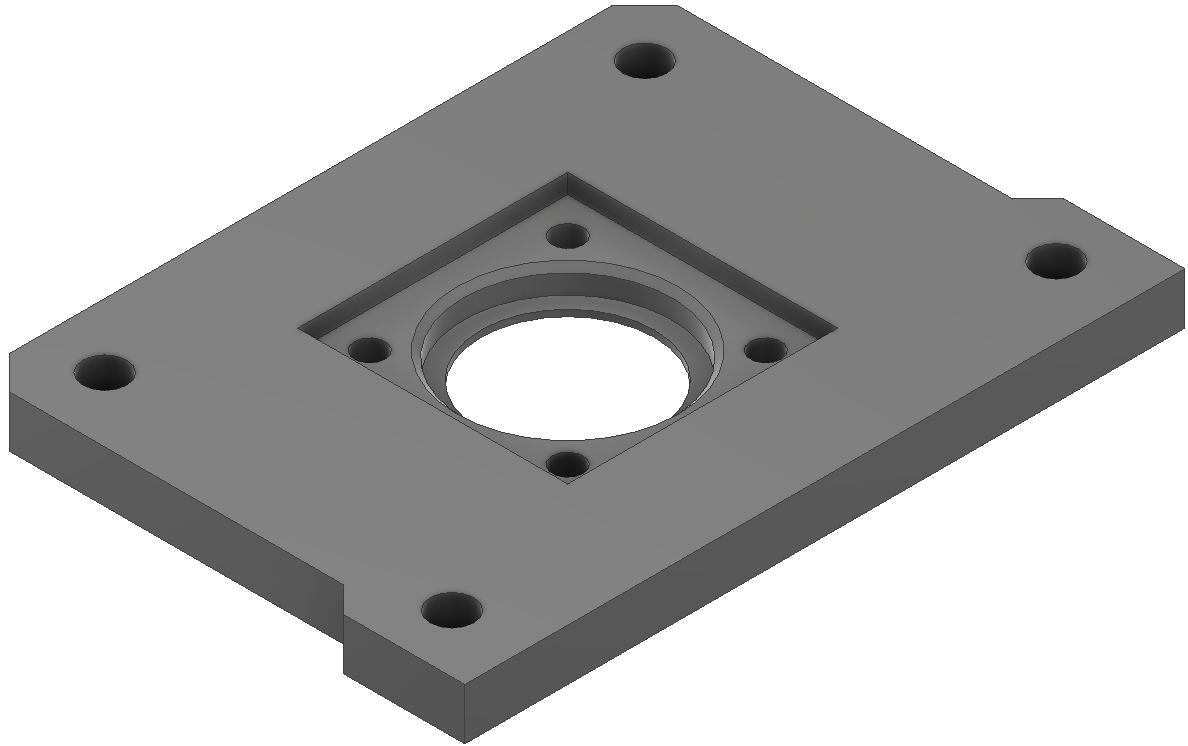
\includegraphics[width=0.65\textwidth]{figures/motor_mount_wide.png}
        \caption{Motorplaat}\label{fig:motorplaat}
    \end{figure}
\end{minipage}\\

\subsection{Loodschroef, motor en askoppeling}\label{sec: motor}
Voor de loodschroef is een schroef van het type T4 gekozen met een spoed en lood van 1mm. Er is een moer gekozen zonder anti-terugslag mechanisme. Terugslag wordt programmatisch geëlimineerd. De moer heeft 3 gaten, van het formaat M3, die gebruikt worden om de geleideslede te bevestigen.
\\[12pt]De motor is een Nema 8 stappermotor van het type 8HS15--0604D met een maximaal koppel van 0.4N-cm en een stapgrootte van 1.8° per stap. De motor heeft vier aansluitingen (twee per fase) en wordt in open lus aangestuurd. Voor nauwkeurigheid wordt aangeraden de pipet regelmatig naar de nulpositie te brengen, waarvoor een eindeloopschakelaar is voorzien.
\\[12pt]De askoppeling is een flexibele askoppeling van het type 4mm-4mm. Er is gekozen voor een flexibele askoppeling omdat, door het stuikgedrag van PLA na het bevestigen van de moeren, de assen niet meer perfect uitgelijnd zijn.

\subsection{Geleideslede}
De geleideslede stuurt de zuiger aan en bestaat uit drie onderdelen. Het centrale deel is met drie M3-schroeven bevestigd aan de moer van de loodschroef. Zoals te zien in \autoref{fig:CarriageDemonstration} zijn later hoge wanden toegevoegd om oscillaties te verminderen, wat succesvol bleek. Dit zorgt voor wat extra weerstand maar deze is niet significant.
\\[12pt]Aan de slede (\autoref{fig:CarriageAndClamp}) is ook een klem bevestigd via 55 mm geleidestaven, gemonteerd zoals bij de hoofdgeleiding. De klem bestaat uit twee delen: een onderste met een gleuf die de zuiger vasthoudt bij de opwaartse beweging, en een bovenste deel dat de zuiger volledig inklemt. Deze delen zijn vervangbaar afhankelijk van de zuigerafmetingen.
\\[12pt]\begin{minipage}[t]{0.39\textwidth}
    \vspace{0pt}
    \begin{figure}[H]
        \centering
        \captionsetup{width=1\textwidth} % wider caption box
        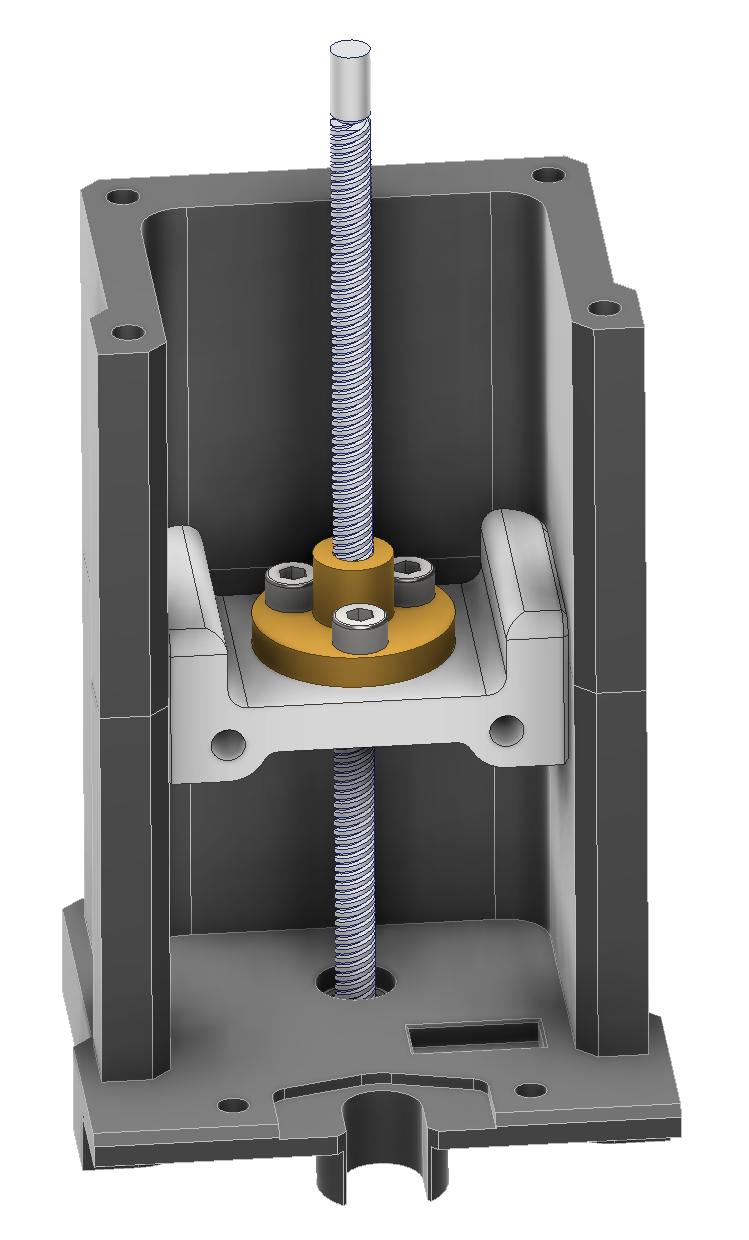
\includegraphics[width=0.65\textwidth]{figures/CarriageDemonstration.png}
        \caption{Geleideslede tussen de wanden}\label{fig:CarriageDemonstration}
    \end{figure}
\end{minipage}
\begin{minipage}[t]{0.59\textwidth}
    \vspace{0pt}
    \begin{figure}[H]
        \centering
        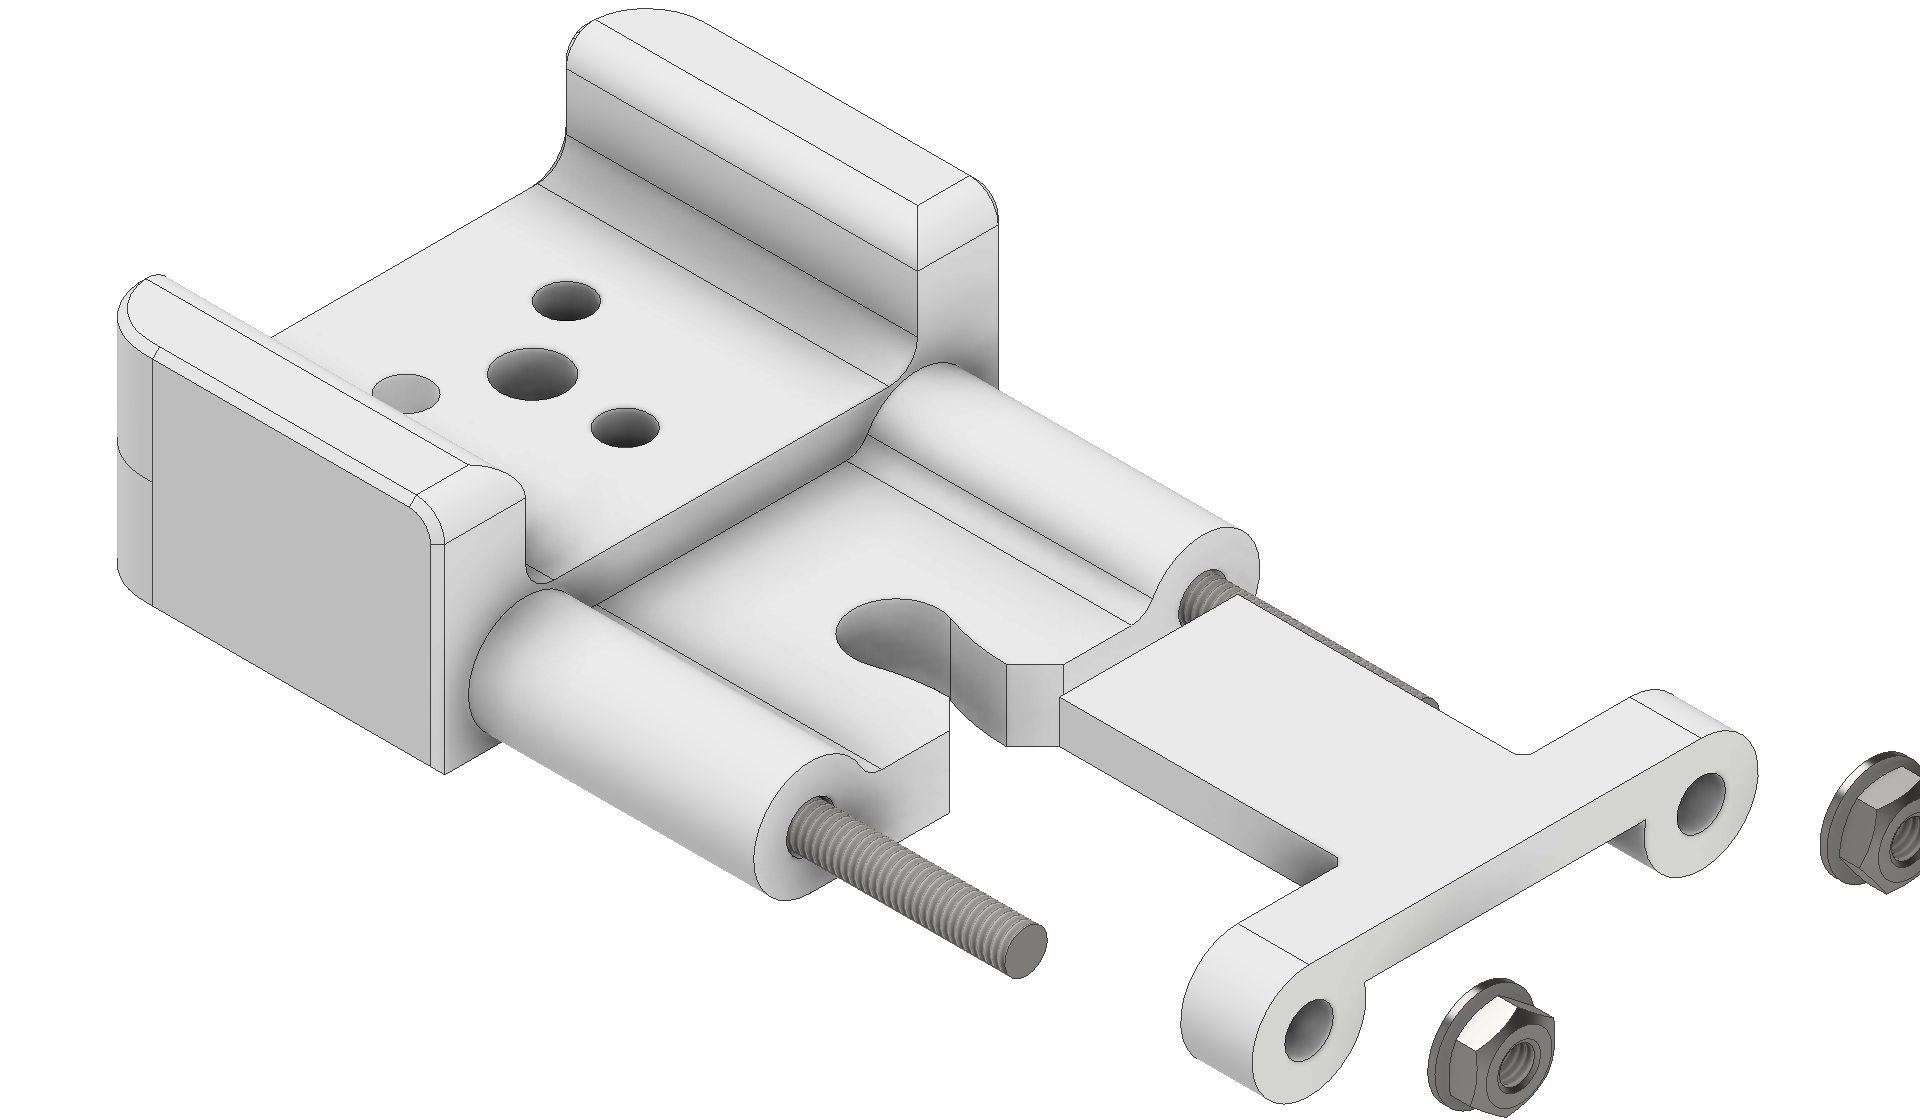
\includegraphics[width=0.85\textwidth]{figures/CarriageAndClamp.png}
        \caption{Geleideslede inclusief de \\samengestelde zuigerklem}\label{fig:CarriageAndClamp}
    \end{figure}
\end{minipage}\\

\subsection{Zuiger}
Voor de zuiger is gekozen voor standaard verkrijgbare spuiten met een volume van 1000 $\mu L$. Deze spuit kan vervangen worden naargelang de gebruikssituatie. In het huidige ontwerp wordt er gebruik gemaakt van met een spuit van het merk BD, type ISO 7886--1 Luer Slip 1ml. Doordat deze spuiten courant beschikbaar zijn, kunnen ze indien nodig vervangen worden.
Een belangrijk aspect bij de keuze voor een bestaande spuit was het feit dat ge-3D-printe onderdelen niet luchtdicht genoeg zijn en dus geen stabiel genoeg vacuüm kan onderhouden. Door een bestaande spuit te gebruiken kan deze bron van fouten deels verholpen worden.


\section{Hardware ontwerp}
Dit onderdeel behandelt de keuzes betreffende de hardware in dit project. De onderdelen die ge-3D-print zijn, werden ontworpen in Autodesk Inventor en geprint met Prusa Mk3S en Prusa Mk4 printers.

\section{Elektronica ontwerp}
\subsection{Componentenlijst}
\begin{minipage}{\linewidth}
    \begin{table}[H]
        \centering
        \caption{Componentenlijst}\label{tab:componentenlijst}
            \centering
            \begin{tabular}{|l|c|c|}
                \hline
                \textbf{Component} & \textbf{Type} & \textbf{Aantal} \\
                \hline
                Motor & Nema 8 (8HS15--0604D) & 1 \\
                Motor driver & BigTreeTech TMC2209 & 1 \\
                Microcontroller & ESP32-WROOM-32 & 1 \\
                Eindeloopschakelaar & Micro Limit switch & 1 \\
                5V Voeding & Vrij te kiezen\footnotemark{} & 1 \\
                \hline
            \end{tabular}
    \end{table}
\footnotetext{{$I_{bron} > 1.7A$}}
\subsection{Driver}
Er is gekozen voor de TMC2209 driver die vooral vanwege de ``StealthChop'' technologie zorgt voor een stille, soepele motorwerking met hogere precisie en minder ruis. Dit is belangrijk voor een constante en nauwkeurige pipetteersnelheid. Daarnaast verhoogt het geoptimaliseerde stroomprofiel het effectieve koppel van de motor\ \cite{RN45}.

\subsection{Microcontroller}
Als microcontroller is de ESP32-WROOM-32 gekozen, dankzij de hoge kloksnelheid (80–240\,MHz, zie\ \cite{RN47}). Dit maakt het mogelijk om zeer snel stap-signalen naar de driver te sturen, wat gunstig is voor nauwkeurige microstepping. Door de hoge klokfrequentie kan de ESP32 de motor sneller aandrijven dan veel andere controllers. Bovendien is de ESP32 betaalbaar (ongeveer €10) en eenvoudig verkrijgbaar.
\subsection{Aansluiting}
De aansluiting gebeurt zoals weergegeven in \autoref{fig:schematische_aansluiting}.
\begin{figure}[H]
    \centering
    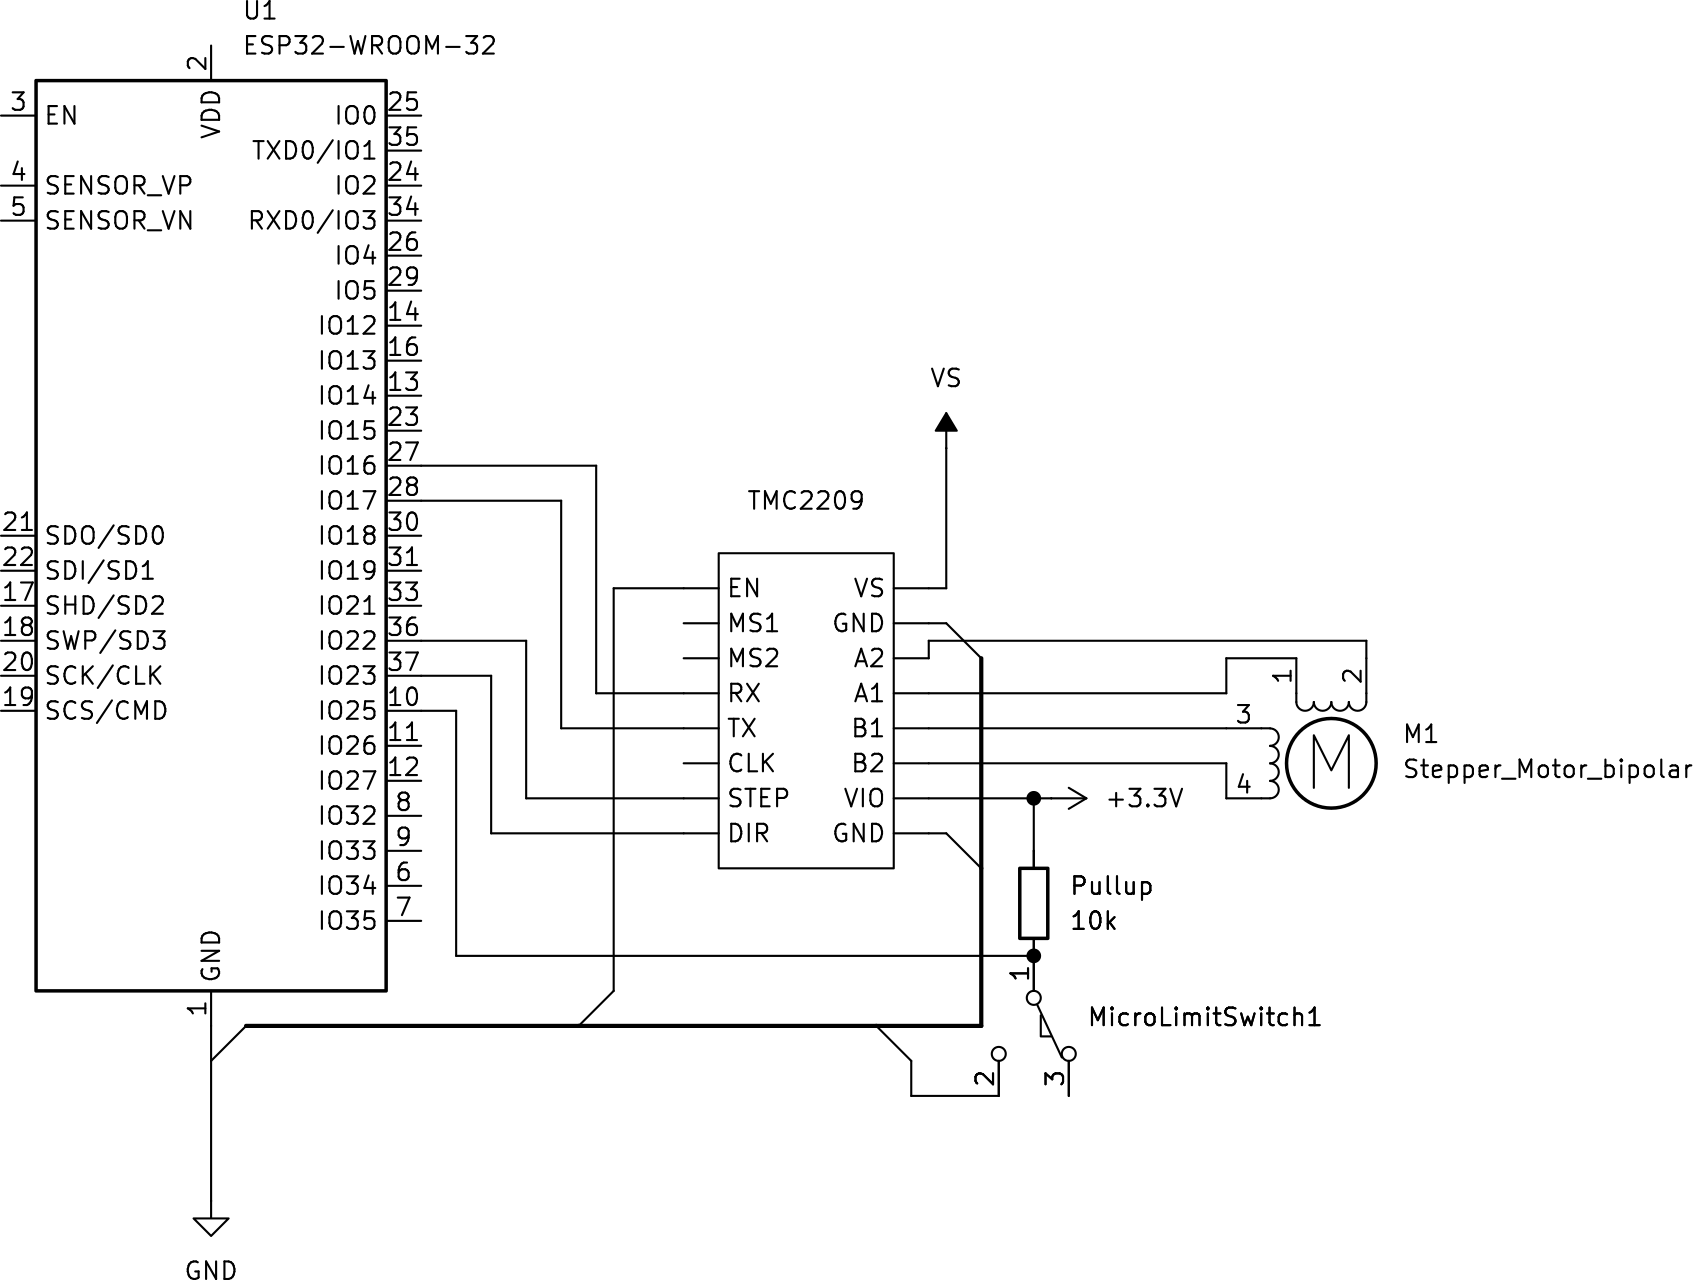
\includegraphics[width=0.85\textwidth]{figures/Wiring_BW.png}
    \caption{Schema van aansluiting}\label{fig:schematische_aansluiting}
    De aansluiting van TX en RX aan de driver is vrijblijvend, maar is wel aangeraden aangezien hiermee de stroomlimiet en microstapgrootte geconfigureerd kunnen worden.
\end{figure}
\end{minipage}

\section{Software ontwerp}

\begin{comment}
\subsection{Overzicht van communicatiepad voor Robot.aspirate(500, 20)} zoals in \autoref{fig:Flowchart}.
\begin{table}[H] \centering 
    \begin{tabular}{l|l|l|p{6cm}} 
        \textbf{Stap} & \textbf{Module / Object} & \textbf{Communicatievorm} & \textbf{Beschrijving} \\
        \hline 
        1 & \texttt{User.py} & Intern (Python) & Aanroep: \texttt{Robot.aspirate(500, 20)} \\
        \hline 
        \multicolumn{4}{c}{\textbf{HTTP-PAD}} \\ 
        \hline 
        H1 & \texttt{HTTPRobotControlAPI.aspirate()} & HTTP POST & Bouwt JSON-object: \texttt{{``volume'': 500, ``rate'': 20}} en stuurt dit naar \texttt{/aspirate} endpoint op de Flask-server \\
        H2 & \texttt{robot\_server.py} (Flask server) & Intern (Python) & Parseert JSON en roept aan: \texttt{robot.aspirate\_pipette(500, 20)} \\
        \hline 
        \multicolumn{4}{c}{\textbf{LOKAAL PAD}} \\
        \hline
        L1 & \texttt{LocalRobotControlAPI.aspirate()} & Intern (Python) & Roept aan: \texttt{robot.aspirate\_pipette(500, 20)}\\ 
        \hline 
        \multicolumn{4}{c}{} \\
        \hline
        3 & \texttt{RobotObject.aspirate\_pipette()} & Seriële commando’s via UART & Vormt ASCII-commando: \texttt{``A500 R20''} en verzendt dit naar de ESP32 \\
        4 & ESP32 (Arduino firmware) & Hardware-instructies & Parseert commando, rekent stappen/rps uit en activeert stepper via TMC2209 \\
        5 & \texttt{ESP -> Python (terug)} & Serieel (UART) & JSON-response: \texttt{\{``status'':``success'', ``message'':``Aspirated X steps at Y rps''\}} terug naar Python \\
    \end{tabular}
    \caption{Communicatieverloop van \texttt{Robot.aspirate(500, 20)} via HTTP en Local.}\label{tab:aspirate_commando} 
\end{table}
\end{comment}
\begin{comment}
\subsection{Belangrijke functionaliteit in de software}
\begin{itemize}
    \item \textbf{Nulzetten van de robot}: elke sessie begint met het nulzetten van de pipet via een eindeloopschakelaar.
    \item \textbf{Veiligheidsgrenzen}: softwarematig worden de minimale en maximale volumes bewaakt.
    \item \textbf{Commandostructuur}: communicatie gebeurt via eenvoudige commando’s zoals ``A500 R20'' (aspireer 500 $\mu l$ aan 20 $\mu l/s$) en ``Z'' (zero).
    \item \textbf{Logging en foutafhandeling}: alle acties en fouten worden gelogd met behulp van colorlog.
\end{itemize}
De software bestaat uit drie lagen: de gebruikersinterface, de middleware (robot control API) en de firmware op de ESP32.\ \autoref{fig:Flowchart} toont het overzicht van de communicatie tussen de verschillende modules.
\end{comment}

\subsection{Opbouw van de software}

Zoals te zien in \autoref{fig:Flowchart} start de gebruiker een sequentie via een Python-script, dat gebruikmaakt van een HTTP-client of een lokale seriële client. De HTTP-client communiceert met een server (bijv.\ op een Raspberry Pi), terwijl de lokale client rechtstreeks communiceert met ``RobotObject''. Beide clients gebruiken dezelfde methodes zoals \texttt{aspirate}, \texttt{dispense} of \texttt{zero\_robot}, maar verschillen in hun onderliggende communicatielaag.
\\[12pt]\begin{figure}[H]
    \centering
    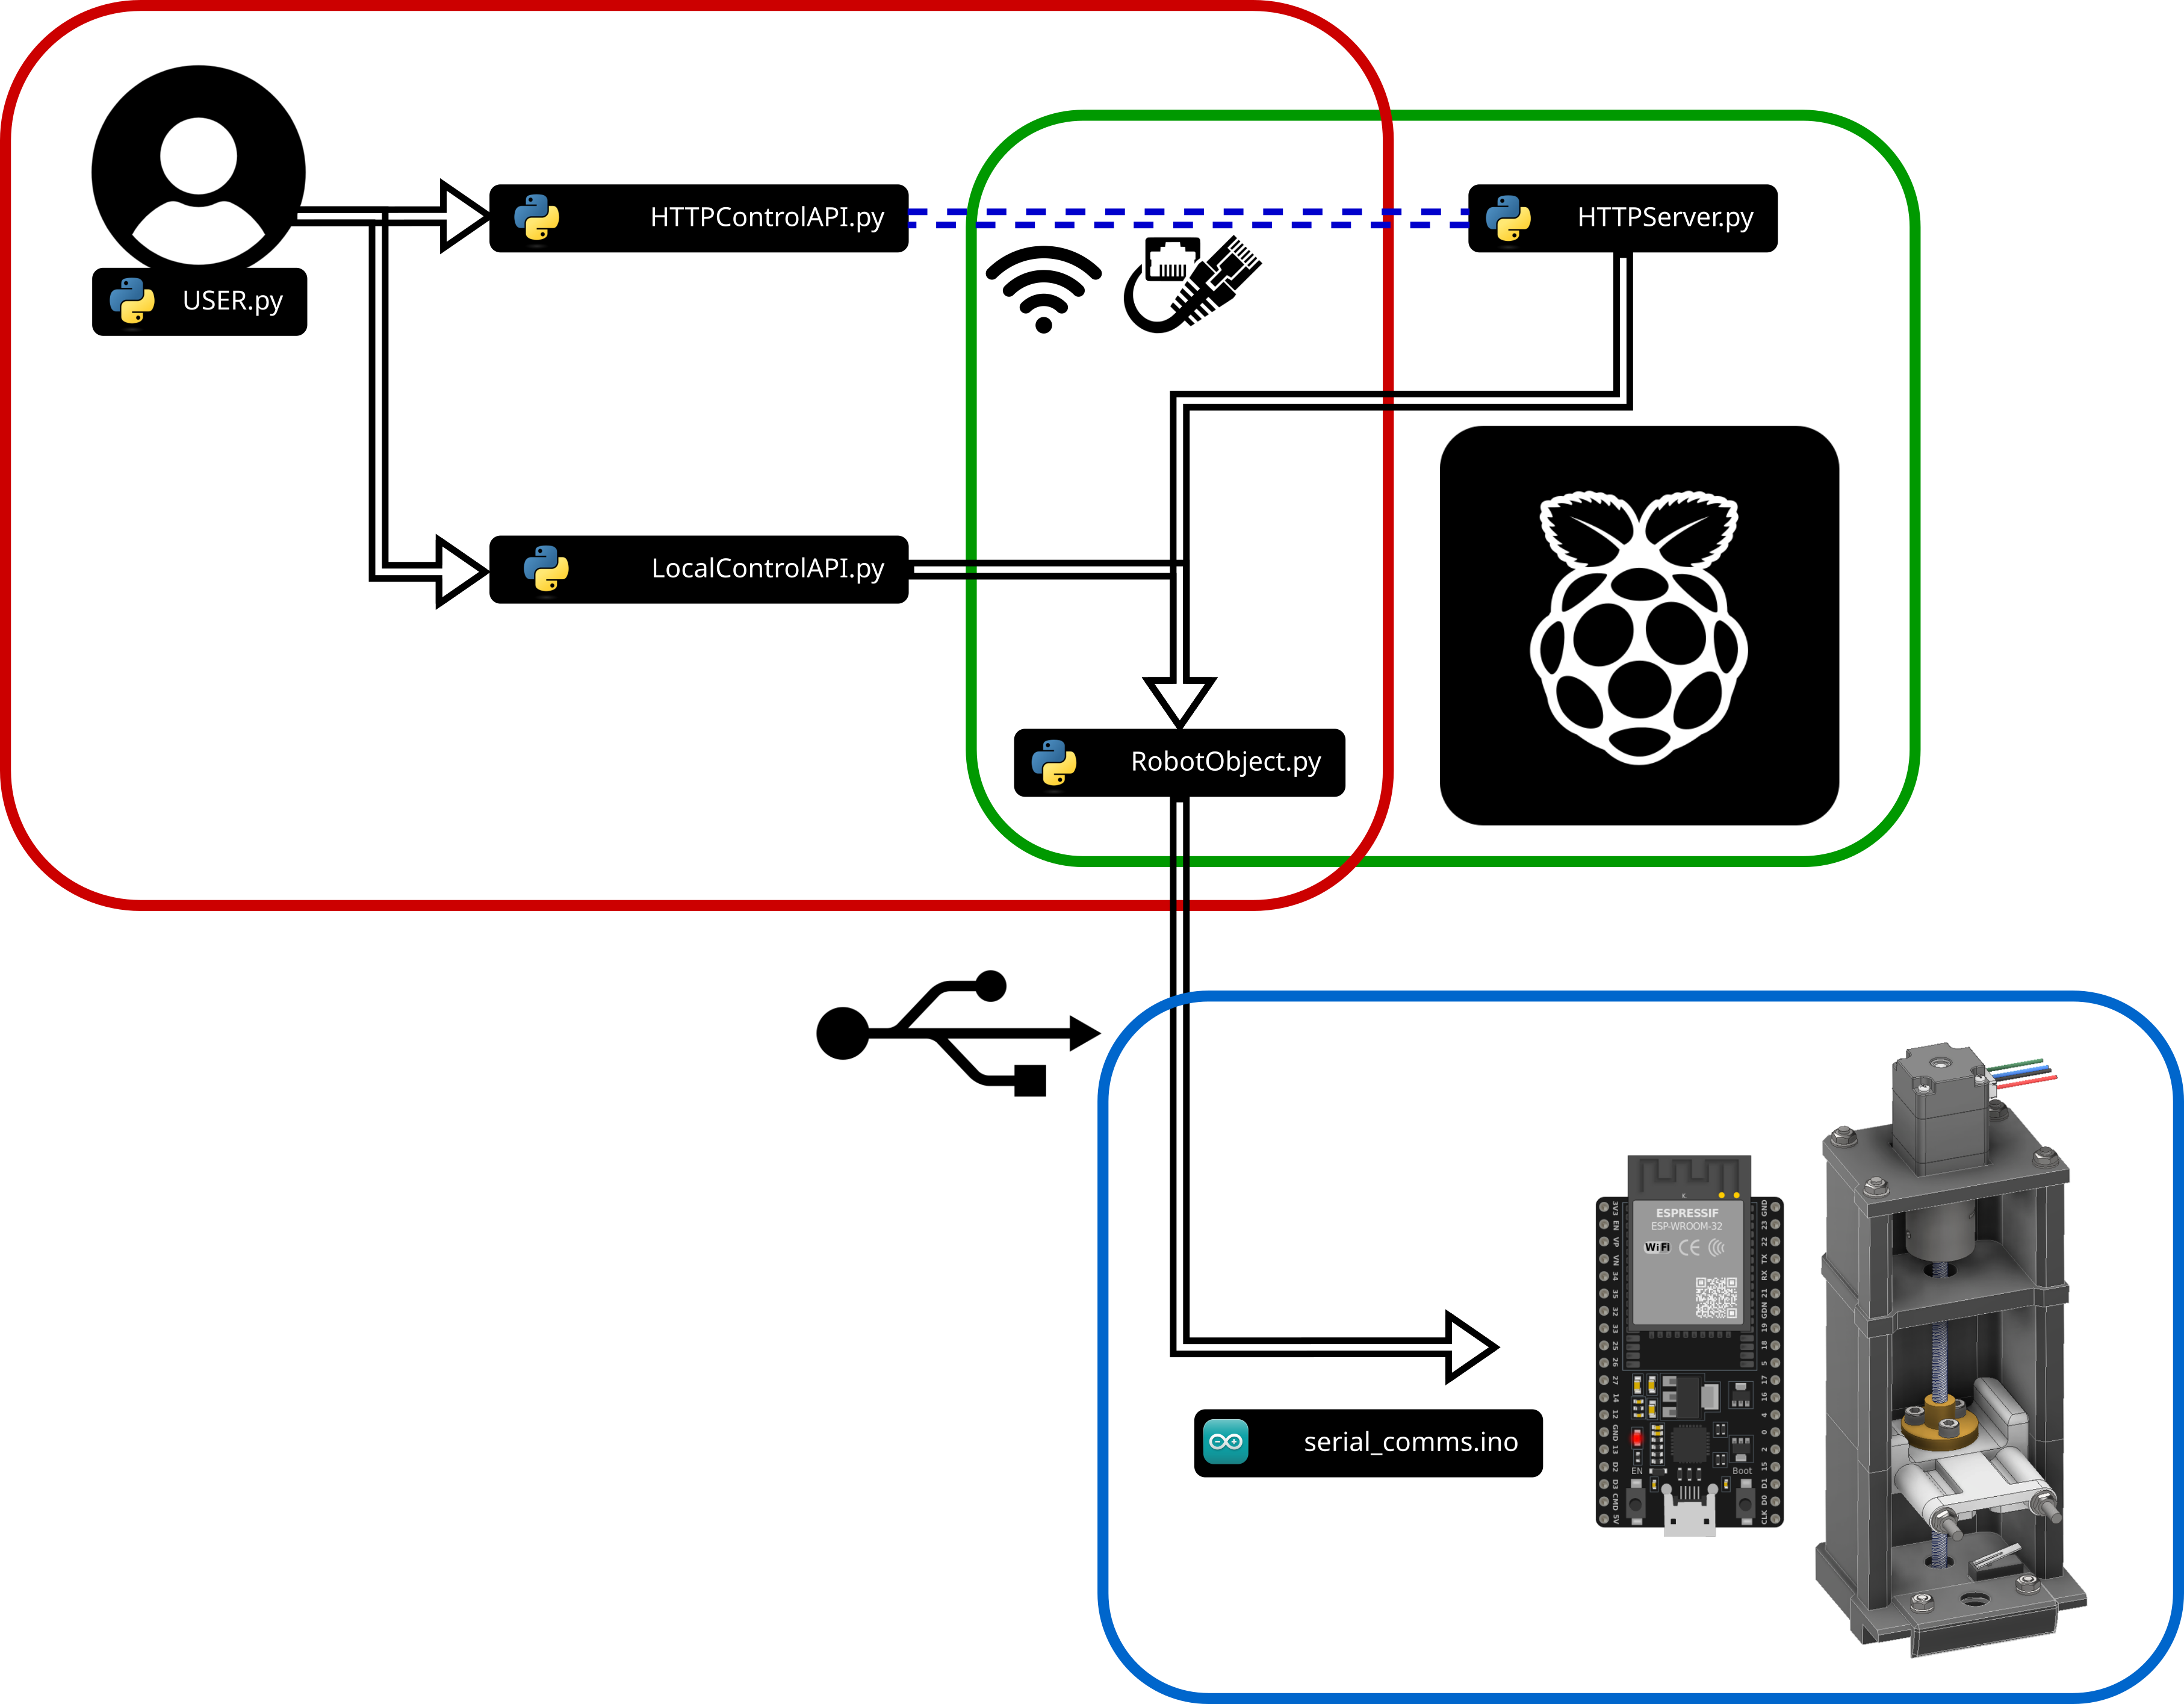
\includegraphics[width=0.85\textwidth]{figures/Flowchart.png}
    \caption{Flowchart communicatie (met als voorbeeld aspireer 500 $\mu L$ aan 20 $\mu L/s$)}\label{fig:Flowchart}
\end{figure}
\vspace{0pt}
De opgeroepen methodes in ``LocalRobotControlAPI'' of ``RobotServer'' sturen de commando's door naar ``RobotObject''. Deze verwerkt het commando en stuurt het via de seriële lijn door naar de microcontroller. Door ``RobotObject'' als een zelfstandig object te definiëren, kan de gebruikersinterface worden aangepast zonder impact op de communicatie met de microcontroller.
\\[12pt]De microcontroller vertaalt de ontvangen commando’s naar motoraansturing via de ESPFlexy-Stepper bibliotheek. Na elke actie stuurt de microcontroller een JSON-respons terug naar de Python-client, die deze logt en indien nodig verder verwerkt.

\begin{comment}
\subsection{Overzicht van software-objecten en communicatiekanalen}
\begin{table}[H] 
    \centering 
    \begin{tabular}{l|l|l|l} 
        \textbf{Object/module} & \textbf{Verantwoordelijkheid} & \textbf{Taal} & \textbf{Communicatie} \\
        \hline 
        \texttt{User.py} & Script gebruiker & Python & HTTP of Serial \\
        \texttt{HTTPRobotControlAPI} & HTTP-client API voor robotaansturing & Python & HTTP (JSON) \\
        \texttt{LocalRobotControlAPI} & Seriële client API voor robotaansturing & Python & Serieel \\
        \texttt{RobotServer} & Flask-server voor HTTP-commando's & Python & Serieel intern \\
        \texttt{RobotObject} & Middleware tussen software en hardware & Python & Serieel \\ 
        \texttt{ESP32 firmware} & Motorbesturing via seriële interface & C++ (Arduino) & ASCII over UART \\
        \texttt{TMC2209 driver} & Motor driver met StealthChop & Hardware & Step/Dir signalen \\
    \end{tabular} 
    \caption{Overzicht van gebruikte softwaremodules en hun communicatie.}\label{tab:software_overzicht} 
\end{table}
\end{comment}

\section{Kalibratie en validatie}
Voor de kalibratie wordt gebruikgemaakt van gravimetrische meting met gedeïoniseerd water en een analytische balans volgens ISO 8655--6\ \cite{RN50}. Deze meting zal op twee verschillende spuiten identiek worden uitgevoerd. Beiden met een spuit van 1000 $\mu L$ om zo een beeld te krijgen op de mogelijke variatie tussen spuiten. De kalibratie wordt uitgevoerd met een analytische balans.
Hierbij wordt het voorbeeld gevolgd van\ \cite{RN49}. Hier wordt ook een spuit-gebaseerd ontwerp getest op nauwkeurigheid met de beschreven procedure.
Elk ingesteld volume (100 $\mu L$, 500 $\mu L$ en 1000 $\mu L$) wordt 10 keer herhaald (per spuit). Deze volumes zijn 10\%, 50\% en 100\% van het nominale volume. 
\\[12pt]De gemeten massa $m_i$ van het opgenomen water wordt omgezet naar volume $V_i$ met behulp van een correctiefactor Z, die afhangt van de temperatuur en de luchtdruk:

\begin{equation} V_i = m_i \cdot Z \end{equation}
\pagebreak
\\Het gemiddelde volume $\bar{V}$ voor n metingen wordt berekend als:

\begin{equation} \bar{V} = \frac{1}{n} \sum_{i=1}^{n} V_i \end{equation}

De systematische fout (nauwkeurigheid) $e_s$ wordt dan gedefinieerd als:

\begin{equation} e_s = \bar{V} - V_s \end{equation}

waarbij $V_s$ het ingesteld doelvolume is. 
\\[12pt]De precisie wordt uitgedrukt als de standaarddeviatie (random error $S_r$) van de metingen:

\begin{equation} S_r = \sqrt{ \frac{1}{n-1} \sum_{i=1}^{n} {(V_i - \bar{V})}^2 } \end{equation}